\documentclass[11pt, oneside]{article}

\usepackage{geometry}            
\geometry{letterpaper}
\usepackage{caption}
\usepackage{authblk}
\usepackage{amssymb}
\usepackage{pst-node}
\usepackage{tikz-cd} 
\usepackage{tikz}
\usepackage{amsmath}
\usepackage{verbatim}
\usetikzlibrary{positioning}
\usepackage{hyperref}
\usepackage{float}
\newcommand{\verbatimfont}[1]{\renewcommand{\verbatim@font}{\ttfamily#1}}

\makeatletter
\g@addto@macro\@floatboxreset\centering
\makeatother

\graphicspath{ {../src/images/}{./images} }

\title{Image Analysis and Computer Vision Homework}
\author{Giorgio Romeo}
\affil{Politecnico di Milano \\ A.Y. 2021/2022}
%\date{}							% Activate to display a given date or no date


\begin{document}
\maketitle

\begin{figure*}[!b]
	\centering
	\includegraphics[width=0.7\linewidth]{Logo_Politecnico_Milano.png}
	\label{logo}
\end{figure*}

\pagebreak
\tableofcontents
\pagebreak

\section{Introduction}
The homework is based on the back side of Villa Melzi d’Eril in Bellagio. In the bottom view below (Fig. \ref{scene}), all lines lie on a same horizontal plane $\Pi$. In addition the facades 1 and 5 are coplanar, and both are parallel to facade 3. Furthermore, facades 2 and 4 are perpendicular to facades 1, 3 and 5. The sun is placed at the point at the infinity
$ S = [3.9\quad \text{-} 1\quad z\quad 0]^\intercal $
-where $z$ is irrelevant- with respect to the reference frame reported in the picture. The layout of the architectonic elements on facade 3 is symmetric with respect to a central vertical axis. Windows of facades 1, 3 and 5 are are equally wide. Windows of facades 2 and 4 can not be exploited in reconstruction since they are poorly visible.

An image of the back side of Villa Melzi d’Eril is taken by a digital camera (Fig. \ref{Villa}). The camera skew factor is assumed to be null; the aspect ratio is unknown (thus natural camera can not be assumed), as well as the principal point and the focal distance. The camera height (z-coordinate) over the ground plane is 1.5 m.\\


\begin{figure}[!h]
\centering
\begin{minipage}{.5\textwidth}
	\centering
	\includegraphics[width=1\linewidth]{scene.png}
	\captionof{figure}{Scene}
	\label{scene}
\end{minipage}%
\begin{minipage}{.5\textwidth}
	\centering
	\includegraphics[width=0.5\linewidth]{Villa.png}
	\captionof{figure}{Back side of Villa Melzi d'Eril}
	\label{Villa}
\end{minipage}
\end{figure}


\section{Feature extraction}
\textbf{Combining the learned techniques, find edges, corner features and straight lines in the image.} \hfill \break
The features were extracted in three steps:
\begin{itemize}
	\item Edge detection using Canny algorithm
	\item Line detection using Hough transform
	\item Corner detection using Harris-Stevens algorithm
	
\end{itemize}

\subsection{Edge detection}
The Canny algorithm relies on a multi-stage edge detector. It can be divided in three steps:
\begin{itemize}
	\item \textit{Computation of the magnitude and angle of the directional gradients}: it uses a filter based on the derivative of a Gaussian in order to compute the intensity of the gradients. The Gaussian reduces the effect of noise present in the image.
	\item \textit{Non-Maximum suppression}: the image magnitude produces results in thick edges but the final image should have thin edges. Thus, to thin out the edges, we perform non-maximum suppression by finding the pixel with the maximum value in an edge
	\item \textit{Hysteresis thresholding}: some edges may not actually be edges and there is some noise in the image. Double thresholding deals with this problem. A pixel is considered an \textit{edge pixel} if its gradient is above "high" threshold, a \textit{non-edge pixel} if its gradient is below "low" threshold. Furthermore, if the gradient at a pixel is between "low" and "high" thresholds then declare it an edge pixel if and only if it can be directly connected to an edge pixel or connected via pixels between "low" and "high".
\end{itemize}
The threshold parameters found for Canny algorithm are the result of many experiments. Note that the line extraction part is affected by this final result.
The processed image with extracted edges is shown in figure \ref{image_edges}.
\begin{figure*}[!h]
	\centering
	\includegraphics[width=0.43\linewidth]{image_edges.png}
	\captionof{figure}{Extracted edges of the image}
	\label{image_edges}
\end{figure*}

\subsection{Line detection}
The Hough transform is a technique that can be used to isolate features of a particular shape within an image. In our case, the Hough transform was used to detect straight lines. Since the Cartesian representation for lines does not include vertical lines, it is more convenient to utilize the parametric notation:
$ rho = x*cos(\theta) + y*sin(\theta) $.

Each datum (edge point extracted using Canny algorithm) votes for all models compatible with it. The followed steps are:
\begin{itemize}
	\item Discretization of the Hough Space into cells
	\item For each cell, set a vote counter equals to 0
	\item For each datum:
		\begin{itemize}
			\item Compute the Hough Transform
			\item Determine cells crossed by Hough Transform
			\item Increment vote counter for crossed cells
		\end{itemize}
	\item Select cells where vote counter is greater than a threshold and is a local max
	\item Refine line estimate by refitting to points that voted that line
\end{itemize}
The result of the application of the Hough Transform for line detection is shown in Fig. \ref{image_lines}.
\begin{figure*}[!h]
	\centering
	\includegraphics[width=0.3766\linewidth]{image_lines.png}
	\captionof{figure}{Extracted lines of the image}
	\label{image_lines}
\end{figure*}


\subsection{Corner detection}
A corner can be interpreted as the junction of two edges, where an edge is a sudden change in image brightness. Harris-Stevens algorithm considers a small window (in our case 3 x 3) around each pixel in the image. We want to identify all pixel windows that are unique, where uniqueness can be measured by shifting each window by a small amount in a given direction and measuring the amount of change that occurs in the pixel values.

We compute the sum squared difference (SSD) of the pixel values before and after the shift and identify pixel windows where the SSD is large for shifts in all 8 directions. We define the change function E(u,v) as the sum of all the SSD, where u,v are the x,y coordinates of every pixel in our 3 x 3 window and I is the intensity value of the pixel. The features in the image are all pixels that have large values of E(u,v) with respect to a pre-defined threshold. The algorithm identifies a corner if the SSD is be large in shifts for all eight directions.

The processed image with extracted corners is shown in figure \ref{image_corners}.\\
\begin{figure*}[!h]
	\centering
	\includegraphics[width=0.45\linewidth]{image_corners.png}
	\captionof{figure}{Extracted corners of the image}
	\label{image_corners}
\end{figure*}


\section{2D reconstruction of a horizontal section}
\textbf{Rectify (2D reconstruct) the horizontal section of the building from the useful selected image lines and features, including vertical shadows. In particular, determine the ratio between the width of facade 2 (or 4) and the width of facade 3.} \hfill \break
We performed 2D reconstruction of the horizontal section of the building utilizing a stratified approach instead of a direct one in order to increase robustness (numerical errors should decrease). The stratified approach consists of performing sequentially an affine reconstruction and a shape reconstruction of the original image. We first computed the affine mapping $H_{affine}$ that maps the original image to its affine reconstruction. Then, we computed the similarity mapping $H_{shape}$ that maps the obtained affine reconstruction to its shape reconstruction. The overall mapping $H_{r}$ that maps the original image to its shape reconstruction can be computed as follows:
$$ H_{r} = H_{shape} * H_{affine} $$
The overall stratified approach can be summarized in the following diagram:\\\\
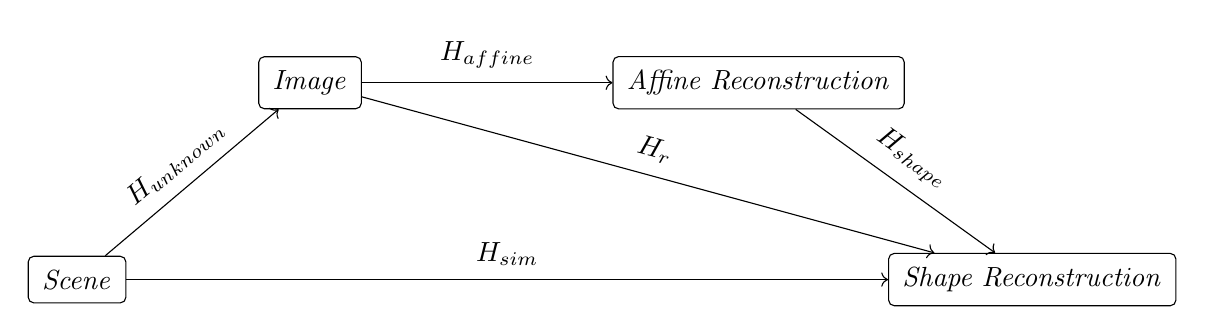
\begin{tikzpicture}[rounded corners=2pt,inner sep=5pt,node distance=0.8cm]
	\node [draw](scene) at (0,0) {\textit{Scene}};
	\node [draw,right=of scene] (image) at (1.5,2.5) {\textit{Image}};
	\node [draw,right=of image] (affine) at (6,2.5){\textit{Affine Reconstruction}};
	\node [draw,right=of affine] (shape) at (9.5,0) {\textit{Shape Reconstruction}};
	\path [->, every node/.style={sloped,anchor=south,auto=false}]
	(scene) edge node {$H_{unknown}$} (image)
	(image) edge node {$H_{affine}$}  (affine)
	(image) edge node {$H_{r}$}  (shape)
	(affine) edge node {$H_{shape}$}  (shape)
	(scene) edge node {$H_{sim}$}  (shape);
\end{tikzpicture}

\subsection{Affine reconstruction}
\label{affine_reconstruction}
An affine transformation is any transformation preserving: parallelism, ratio of areas, ratio of length on collinear or parallel lines, linear combination of vectors, line at the infinity, invariants of a projective transformation. To compute $H_{affine}$ we exploited the fact that a projective mapping $H$ maps the line at the infinity $l_{\infty} = [0\quad0\quad1]^\intercal$ onto itself if and only if $H$ is affine. Thus, this mapping must map any point $x'$ belonging to	$l'_{\infty}$ (image of the $l_{\infty}$) onto a point at the infinity, namely:\\

\begin{equation}
	H_{affine} \; x' = 
	\begin{bmatrix}
		* \\ * \\ 0
	\end{bmatrix}
	\Rightarrow
	\begin{bmatrix}
		* & * & * \\ * & * & * \\ & {l'}^{\intercal}_{\infty} &
	\end{bmatrix}
	\: x' =
	\begin{bmatrix}
		* & * & * \\ * & * & * \\ & {l'}^{\intercal}_{\infty} \; x' &
	\end{bmatrix}
	=
	\begin{bmatrix}
		* \\ * \\ 0
	\end{bmatrix}
\end{equation}

Taking into account that $H_{affine}$ should have the previous form and be non-singular, we chose the following matrix representation (the simplest one):
\begin{equation}
	H_{affine} =
	\begin{bmatrix}
		1 & 0 & 0 \\ 0 & 1 & 0 \\ & {l'}^{\intercal}_{\infty} &
	\end{bmatrix}
	=
	\begin{bmatrix}
		1 & 0 & 0 \\ 0 & 1 & 0 \\ -0.00000795 & -0.00082198 & 1
	\end{bmatrix}
\end{equation}

For the computation of the line at the infinity $l'_{\infty}$, we exploited the blue points highlighted in Fig. \ref{image_original_lines} (the green points were utilized in the shape reconstruction). First of all, we considered an horizontal plane parallel to the floor highlighting the blue points $a, b, c \, \text{and}\, d$. Afterwards, we computed the first vanishing point $vp1$ (not represented in the figure) as the intersection of the two lines $ab$ and $dc$ (images of parallel lines in the real scene), while the second vanishing point $vp2$ as the intersection of the two lines $ad$ and $bc$ (images of parallel lines in the real scene). Eventually, we computed $l'_{\infty}$ as the cross product of the two vanishing points (they belong to the image of the line at the infinity), obtaining the mapping $H_{affine}$ as previously stated. Note that "line $ab$" should be properly defined as "line passing through point $a$ and $b$" (similar for all other lines).

The resulting affine reconstruction obtained applying $H_{affine}$ to the original image is shown in Fig. \ref{image_affine_reconstruction}. Note that the affine transformation $H_{affine}$ was also applied to the blue $(a, b, c, d)$ and green $(g)$ points to represent them in the affine reconstruction.

\begin{figure}[!h]
	\centering
	\begin{minipage}{.40\textwidth}
		\centering
		\includegraphics[scale = 0.35]{image_original_lines.png}
		\captionof{figure}{Features and lines in the original image used for affine and shape reconstruction}
		\label{image_original_lines}
	\end{minipage}%
	\quad
	\begin{minipage}{.55\textwidth}
		\centering
		\includegraphics[scale = 0.35]{image_affine_reconstruction.png}
		\captionof{figure}{Affine reconstruction of the original image}
		\label{image_affine_reconstruction}
	\end{minipage}
\end{figure}
\pagebreak

\subsection{Shape reconstruction} \label{shape_reconstruction}
A similarity transformation is any transformation preserving: ratio of length, angles, circular points, invariants of both projective and affine transformations. To compute $H_{shape}$ we exploited the fact that a projective mapping $H$ maps the circular points $\textbf{I}$ and $\textbf{J}$ onto themselves if and only if $H$ is  a similarity. A crucial property is that, after an affine reconstruction, the dual conic $C^{*'}_\infty$ image of the (original) conic dual to the circular points $(\textbf{I},\textbf{J})$ can be written as:
\begin{equation}
	C^{*'}_\infty = 
	\begin{bmatrix}
		KK^\intercal  & 0 \\ 0^\intercal & 0
	\end{bmatrix}
\end{equation}
where $K$ is a 2 x 2 invertible matrix. $S = KK^\intercal$ is a symmetric and homogeneous matrix, thus there are only 2 unknowns to identify $C^{*'}_\infty$. We found the first unknown exploiting known angles: given two lines $l = [l_1\quad l_2 \quad l_3]^\intercal$ and $m = [m_1\quad m_2 \quad m_3]^\intercal$, the term $l_1 m_1 + l_2 m_2$ can be written as:
\begin{equation}
	\begin{bmatrix}
		l_1 & l_2 & l_3
	\end{bmatrix}
	*
	\begin{bmatrix}
		1 & 0 & 0 \\ 0 & 1 & 0 \\ 0 & 0 & 0
	\end{bmatrix} *
	\begin{bmatrix}
		m_1 \\ m_2 \\ m_3
	\end{bmatrix}
	= l^\intercal C^{*}_\infty m
\end{equation}
Furthermore, from the transformation rules we can derive: $l^\intercal C^{*}_\infty m = l{'^\intercal} C^{*'}_\infty m'$. Thus, we may compute the angle $\theta$ between two lines as:
\begin{equation}
	\label{eqn:angle}
	\cos(\theta) = \frac{l_1 m_1 + l_2  m_2}{\sqrt{(l_1^2 + l_2^2)(m_1^2 + m_2 ^2)}}
	=
	\frac{l^\intercal C^{*}_\infty m}{\sqrt{(l^\intercal C^{*}_\infty l)(m^\intercal C^{*}_\infty m)}} 
	= 
	\frac{l{'^\intercal} C^{*'}_\infty m'}{\sqrt{(l^{'\intercal} C^{*'}_\infty l')(m^{'\intercal} C^{*'}_\infty m')}}
\end{equation}
Referring to Fig. \ref{image_affine_reconstruction}, we selected the pair of lines ad and dc (images of orthogonal lines in the real scene) to exploit the fact that $\cos(\theta) = 0$ for orthogonal lines. Thus, equation (\ref{eqn:angle}) can be simplified as follows:
\begin{equation}
	\label{eqn:constraint_1}
	\cos(\theta) = 0 =
	\frac{l{'^\intercal} C^{*'}_\infty m'}{\sqrt{(l^{'\intercal} C^{*'}_\infty l')(m^{'\intercal} C^{*'}_\infty m')}} 
	\Rightarrow
	l{'^\intercal} C^{*'}_\infty m' = 0
\end{equation}
More specifically, we wrote equation (\ref{eqn:constraint_1}) as:
\begin{equation}
	\begin{bmatrix}
		l_1 & l_2 & l_3
	\end{bmatrix}
	*
	\begin{bmatrix}
		a & b & 0 \\ b & c & 0 \\ 0 & 0 & 0
	\end{bmatrix} *
	\begin{bmatrix}
		m_1 \\ m_2 \\ m_3
	\end{bmatrix}
	= l_1 m_1 a + l_2 m_1 b + l_1 m_2 b + m_2 l_2 c = 0
\end{equation}
Eventually, we obtained the first constraint:
\begin{equation}
	\begin{bmatrix}
		l_1 m_1 & l_1 m_2 + l_2 m_1 & l_2 m_2
	\end{bmatrix}
	*
	\begin{bmatrix}
		a \\ b \\ c
	\end{bmatrix}
	= 0
\end{equation}

Note that we could not select another pair of orthogonal lines such as $dc$ and $cb$ for the second constraint because this one would not have been independent from the previous constraints. For the last constraint, we exploited the invariance of ratio of length in similarity transformations.

First of all, as shown in Fig. \ref{scene_triangles}, exploiting the fact that the sun is a point at the infinite along the direction $[3.9\quad\text{-}1]$ ($z$ is irrelevant) and triangles 1 and 2 are similar (same angles), we computed the ratio $k$ between the lengths of segments $gd$ and $ad$: $k = 1/3.9$. Segment $ad$ represents the width of facade 2, while $gd$ represents the width of the shadow segment defined from point $d$ (junction of facade 2 and 3) and point $g$ (intersection of the vertical shadow $eg$ and the plane defined by the blue points $(a, b, c, d)$, as shown in Fig. \ref{image_original_lines}).
The two segments were computed as:
\begin{equation}
	gd = 
	\begin{bmatrix}
		g'_1 - d'_1 \\ g'_2 - d'_2 \\ g'_3 - d'_3
	\end{bmatrix}
	=
	\begin{bmatrix}
		l'_1 \\ l'_2 \\ l'_3
	\end{bmatrix}
	= l' , \quad
	ad = 
	\begin{bmatrix}
		a'_1 - d'_1 \\ a'_2 - d'_2 \\ a'_3 - d'_3
	\end{bmatrix}
	=
	\begin{bmatrix}
		m'_1 \\ m'_2 \\ m'_3
	\end{bmatrix}
	= m'
\end{equation}
Furthermore, exploiting the fact that $l/m = 1/3.9 = k$, we computed:
\begin{equation}
	\label{eqn:ratio}
	l_1^{'2} + l_2^{'2} = k^2 (m_1^{'2} + m_2^{'2})
	\Rightarrow
	l^{'\intercal} C^{*'}_\infty l' = k^2 (m^{'\intercal} C^{*'}_\infty m')
\end{equation}
More specifically, we wrote equation (\ref{eqn:ratio}) as:
\begin{equation}
	\begin{bmatrix}
		l_1^{'2} & 2 l'_1 l'_2 & l_2^{'2}
	\end{bmatrix}
	*
	\begin{bmatrix}
		a \\ b \\ c
	\end{bmatrix}
	= k^2
	\begin{bmatrix}
		m_1^{'2} & 2 m'_1 m'_2 & m_2^{'2}
	\end{bmatrix}
	*
	\begin{bmatrix}
		a \\ b \\ c
	\end{bmatrix}
\end{equation}
Eventually, we obtained the second constraint:
\begin{equation}
	\begin{bmatrix}
		l_1^{'2} - k^2 m_1^{'2} & 2 (l'_1 l'_2 - k^2 m'_1 m'_2) & l_2^{'2} - k^2 m_2^{'2}
	\end{bmatrix}
	*
	\begin{bmatrix}
		a \\ b \\ c
	\end{bmatrix}
	= 0
\end{equation}
Once we found the image of the dual conic $C^{*'}_\infty$, using the single value decomposition (SVD) method, we computed:
\begin{equation}
	SVD(C^{*'}_\infty) = U D V^\intercal = H_{shape}^{-1} C^*_\infty H_{shape}^{-1\intercal}
\end{equation}
However, since we did not obtain:
\begin{equation}
	D = C^*_\infty =
	\begin{bmatrix}
		1 & 0 & 0 \\ 0 & 1 & 0 \\ 0 & 0 & 0
	\end{bmatrix}
\end{equation}
we exploited the fact that:
\begin{equation}
	D =
	\begin{bmatrix}
		\sqrt{D_{11}} & 0 & 0 \\ 0 & \sqrt{D_{22}} & 0 \\ 0 & 0 & 0
	\end{bmatrix}
	\begin{bmatrix}
		1 & 0 & 0 \\ 0 & 1 & 0 \\ 0 & 0 & 0
	\end{bmatrix}
	\begin{bmatrix}
		\sqrt{D_{11}} & 0 & 0 \\ 0 & \sqrt{D_{22}} & 0 \\ 0 & 0 & 0
	\end{bmatrix}
	= D_S C^*_\infty D_S
\end{equation}
obtaining:
\begin{equation}
	U D V^\intercal = U D_S C^*_\infty D_S V^\intercal
\end{equation}
Eventually, we computed:
\begin{equation}
	H_{shape} = (U D_S)^{-1} = 
	\begin{bmatrix}
		1.17870261 & -0.24436278 & 0 \\
		-0.24436278 & 1.42341806 & 0 \\
		0 & 0 & 1
	\end{bmatrix}
\end{equation}
The resulting shape reconstruction obtained applying $H_{shape}$ to the affine reconstruction is shown in Fig. \ref{image_shape_reconstruction}. Note that the shape transformation $H_{shape}$ was also applied to the blue $(a, b, c, d)$ and green $(g)$ points to represent them in the shape reconstruction.

Eventually, we computed the overall mapping $H_r$ as:
\begin{equation}
	H_{r} = H_{shape} * H_{affine} =
	\begin{bmatrix}
		1.17870261 & -0.24436278 & 0 \\
		-0.24436278 & 1.42341806 & 0 \\
		-0.00000795 & -0.00082198 & 1
	\end{bmatrix}
\end{equation}


\begin{figure}[!h]
	\centering
	\begin{minipage}{.45\textwidth}
		\centering
		\includegraphics[scale = 0.75]{scene_triangles.png}
		\captionof{figure}{Similar triangles}
		\label{scene_triangles}
	\end{minipage}%
	\quad
	\begin{minipage}{.5\textwidth}
		\centering
		\includegraphics[scale = 0.275]{image_affine_reconstruction.png}
		\captionof{figure}{shape reconstruction of the horizontal section of the buiding}
		\label{image_shape_reconstruction}
	\end{minipage}
\end{figure}

\subsection{Ratio results}
The final task of this point was to compute the ratio between the width of facade 3 and width of facade 3. Thus, referring to Fig. \ref{image_shape_reconstruction}, we measured the length of segment $ad$ (width facade 2) and length of segment $dc$ (width facade 3), obtaining:
$$\frac{Facade\_2_{width}}{Facade\_3_{width}} = 0.659764$$
Even if not required, we also computed the ratio between the width of facade 3 and width of the shadow segment $dg$, both after affine and shape reconstruction. We obtained the same result (invariance of the ratio of length):
$$\frac{Facade\_3_{width}}{Shadow\_Segment_{width}} = 6.891124$$


\section{Calibration}
\textbf{First extract a vertical vanishing point and then use it together with useful information extracted during the rectification step, in order to estimate the calibration matrix $K$ containing the intrinsic parameters of the camera, namely: focal distance, aspect ratio and position of principal point.} \hfill \break
Calibration matrix $K$ is defined as:
\begin{equation} \label{keq}
	K =
	\begin{bmatrix}
		f_x  && 0 && u_0 \\ 0 && f_y && v_0 \\ 0 && 0 && 1
	\end{bmatrix}
\end{equation}
The relation between the image of the absolute conic $\omega$ and the calibration matrix $K$ is:
\begin{equation}
	\label{eqn:omega_K}
	\omega = (KK^t)^{-1}
\end{equation}
Furthermore, for a zero skew camera $\omega$ is given by:
\begin{equation}
	\label{eqn:omega}
	\omega = 
	\begin{bmatrix}
		\alpha^2 && 0 && -u_0 \alpha^2 \\ 0 && 1 && -v_0 \\  -u_0 \alpha^2 && -v_0 && f_y^2 +\alpha^2 u_0^2 + v_0^2
	\end{bmatrix}
\end{equation}
that is a symmetric matrix with 4 degrees of freedom, hence just 4 constraints on $\omega$ were required. For computing the constraints we needed:
\begin{itemize}
	\item the overall mapping $ H_{r} = H_{shape} * H_{affine} $
	\item the image of the line at the infinity $l'_\infty$ (see section \ref{affine_reconstruction})
	\item the vanishing point $vp_{vertical}$ along the direction orthogonal to the horizontal plane defined by points $(a, b, c, d)$ (see Fig. \ref{image_original_lines}). In particular, referring to Fig. \ref{image_original_vertical_vp}, we computed the vertical vanishing point as the intersection between lines $he$ and $gf$ (images of parallel lines in the real scene). 
\end{itemize}
The constraints were computed exploiting:
\begin{itemize}
	\item the image of the circular point $\textbf{I}'$:
	\begin{equation}
		\textbf{I}' = H_r^{-1} \textbf{I} =
		\begin{bmatrix}
			h_1 & h_2 & h_3
		\end{bmatrix}
		\begin{bmatrix}
			1 \\ i \\ 0
		\end{bmatrix}
		= h_1 + ih_2
		\quad \text{and} \quad (h_1 + ih_2)^\intercal \omega (h_1 + ih_2) = 0	
	\end{equation}
	leading to constraints:
	\begin{equation}
		h_1^\intercal \omega h_2 = 0 \quad \text{and} \quad h_1^\intercal \omega h_1 = h_2^\intercal \omega h_2
	\end{equation}
	\item the line at infinity on the horizontal plane is orthogonal with respect to the vanishing point of the vertical direction:
	\begin{equation} \label{eqn:line_vp}
		[l'_{\infty}]_\times\; \omega\; vp_{vertical} = 0
	\end{equation}
	where $[l'_{\infty}]_\times$ is the vector product matrix of $l'_{\infty}$.
	\item the orthogonality of vanishing points belonging to orthogonal directions (such as the ones computed in section \ref{affine_reconstruction}):
	\begin{equation}
		vp_1\; \omega\; vp_2 = 0
	\end{equation}
\end{itemize}
\begin{figure*}[!h]
	\centering
	\includegraphics[width=0.30\linewidth]{image_original_vertical_vp.png}
	\captionof{figure}{Lines to compute the vertical vanishing point}
	\label{image_original_vertical_vp}
\end{figure*}
Once we obtained the image of the absolute conic $\omega$, we computed the calibration matrix $K$ exploiting relation (\ref{eqn:omega}):
\begin{equation}
	K =
	\begin{bmatrix}
		1273.58016001317 & 0 & 540.535823296631 \\
		0 & 975.253444381331 & 875.511631430140 \\
		0 & 0 & 1
	\end{bmatrix}
\end{equation}
where
$$f_x = 1273.58016001317$$
$$f_y = 975.253444381331$$
$$u_0 = 540.535823296631$$
$$v_0 = 875.511631430140$$


\section{Reconstruction of a vertical facade}
\textbf{Use the knowledge of K to rectify also a vertical facade, as, e.g., facade 3.} \hfill \break
Knowing the calibration matrix $K$ we computed the image of the absolute conic as:
\begin{equation}
	\omega = (KK^t)^{-1}
\end{equation}
Referring to Fig. \ref{image_two_original_vertical_vp}, we computed the first vertical (along the vertical direction) vanishing point $vp3$ ($vp_{vertical}$ in equation (\ref{eqn:line_vp})) as the intersection between lines $he$ and $gf$ (images of parallel lines in the real scene) and the second vertical vanishing point $vp4$ as the intersection between lines $hg$ and $ef$ (images of parallel lines in the real scene).

Since the absolute conic contains all the circular points, i.e. the circular points $\textit{I}_\pi$, $\textit{J}_\pi$ of any plane belong to the absolute conic, the image $\omega$ of the absolute conic contains the image $\textit{I}'_\pi$, $\textit{J}'_\pi$ of all the circular points $\textit{I}_\pi$, $\textit{J}_\pi$. Thus, we computed the image of the circular points of the vertical plane (facade 3) as the intersection between the image of the absolute conic $\omega$ and the image of the line at the infinity to which vertical vanishing points vp3 and vp4 belong. Afterwards, we computed the dual conic $C^{*'}_\infty$ image of the (original) conic dual to the circular points $(\textbf{I},\textbf{J})$ as:
\begin{equation}
	C^{*'}_\infty = \textbf{I}' \textbf{J}^{'\intercal} + \textbf{J}' \textbf{I}^{'\intercal}
\end{equation}
Once we found the image of the dual conic $C^{*'}_\infty$, using the single value decomposition (SVD) method, we computed:
\begin{equation}
	SVD(C^{*'}_\infty) = U D V^\intercal = H_{rect}^{-1} C^*_\infty H_{rect}^{-1\intercal}
\end{equation}
As what we did in section \ref{shape_reconstruction}, we exploited the fact that:
\begin{equation}
	D =
	\begin{bmatrix}
		\sqrt{D_{11}} & 0 & 0 \\ 0 & \sqrt{D_{22}} & 0 \\ 0 & 0 & 0
	\end{bmatrix}
	\begin{bmatrix}
		1 & 0 & 0 \\ 0 & 1 & 0 \\ 0 & 0 & 0
	\end{bmatrix}
	\begin{bmatrix}
		\sqrt{D_{11}} & 0 & 0 \\ 0 & \sqrt{D_{22}} & 0 \\ 0 & 0 & 0
	\end{bmatrix}
	= D_S C^*_\infty D_S
\end{equation}
obtaining:
\begin{equation}
	U D V^\intercal = U D_S C^*_\infty D_S V^\intercal
\end{equation}
Eventually, we computed the rectification homography as:
\begin{equation}
	H_{rect} = (U D_S)^{-1}
\end{equation}
The result of the reconstruction of vertical facade 3 are shown in Fig. \ref{image_rectification_vertical_facade}, where we also represented the green points highlighted in the original image in Fig. \ref{image_two_original_vertical_vp}.

\begin{figure}[!h]
	\centering
	\begin{minipage}{.45\textwidth}
		\centering
		\includegraphics[scale = 0.4]{image_original_two_vertical_vp.png}
		\captionof{figure}{Lines used to compute the two vertical vanishing points}
		\label{image_two_original_vertical_vp}
	\end{minipage}%
	\quad
	\begin{minipage}{.5\textwidth}
		\centering
		\includegraphics[scale = 0.4]{image_rectification_vertical_facade.png}
		\captionof{figure}{Reconstruction of facade 3}
		\label{image_rectification_vertical_facade}
	\end{minipage}
\end{figure}
\pagebreak

\section{Localization}
\textbf{Determine the relative pose (i.e. position and orientation) between facade 3 and the camera reference. Use information about the camera height to solve for scale.} \hfill \break
Finding the relative pose between facade 3 (highlighted through points $(e, f, g, h)$ in Fig. \ref{image_rectification_vertical_facade}) and the camera reference was possible knowing the size and shape of facade 3, the image and the calibration matrix $K$.

Identifying the plane of the vertical facade 3 with $\pi$ and the position of a point in the plane reference frame with $X_{\pi}$, we can write the position of a point in the world reference frame as:
\begin{equation}
	 X_w =[R_{\pi} | o_{\pi}]X_{\pi} 
\end{equation} 
Referring to Fig. \ref{image_rectification_vertical_facade}, the plane reference frame has the y axis identical to the line at the bottom of facade 3, going right, the z axis with the same direction of the left line $he$ and the x axis orthogonal to both axis using the right hand rule. Thus, the origin of the plane reference frame is represented by point $h$.
In this way a point on the plane can be written (in homogeneous coordinates) as:
\begin{equation}
	X_\pi = 
	\begin{bmatrix}
		0 \\ y \\ z \\ w
	\end{bmatrix}
\end{equation}
Defining as $P$ the projection matrix:
\begin{equation} \label{peq}
	P=[KR | -KRo]
\end{equation}
mapping 3D points ($X$) of the world to points in the image ($x$). From:
\begin{equation} \label{peq1}
	x = P X
\end{equation}
we obtained:
\begin{equation}
	u = [KR | -KRo] [R_{\pi} | o_{\pi}]X_{\pi}
\end{equation}
By putting the world reference frame on the camera ($R=I$ and $o=[0 \ 0\ 0]^\intercal$):
\begin{equation}
	u = [K|\underline{\mathbf{0}}]
	\begin{bmatrix}
		j_\pi & k_\pi & o_\pi \\ 0 & 0 & 1
	\end{bmatrix}
	\begin{bmatrix}
		y \\ z \\ w
	\end{bmatrix}
	\Rightarrow
	u = K [j_\pi | k_\pi | o_\pi] x
\end{equation}
Where x are the coordinates of the point on the plane. By inspection we identified $K [j_\pi | k_\pi | o_\pi] = H_{homography}$ the matrix that maps the real points to the image. $H$ was known since we knew shape and size of facade 3 (transformation mapping the shape of facade 3 face to the image).
So we obtained:
\begin{equation}
	[j_\pi | k_\pi | o_\pi]= K^{-1}H_{homography} 
\end{equation}
Where $H_{homography} = [h_1\; |\; h_2\; |\; h_3]$ is the transformation mapping world points to image points. The matrix $R=[i_\pi\; | \; j_\pi \; | \; k_\pi]$ (rotation of the plane with respect to the camera) can be found using these equations:
\begin{subequations}
	\begin{align*}
		\lambda &= \frac{1}{|K^{-1}h_1|} \\
		j_\pi &= K^{-1}h_1\lambda \\
		k_\pi &= K^{-1}h_2\lambda \\
		i_\pi &= j_\pi \times k_\pi  \\
		o_\pi &= K^{-1} h_3 \lambda
	\end{align*}
\end{subequations}
Due to noise in the data R may be not a true rotation matrix, thus, we approximated it through SVD, obtaining an orthogonal matrix:
\begin{equation}
	SVD(R) = [U,\; \sim\;,\;V] \Rightarrow \hat{R} = UV
\end{equation}
The computed camera position and camera rotation are:
\begin{subequations}
	\begin{align*}
	cameraPosition &=
	\begin{bmatrix}
		17.96874075 \\ 2.41349869 \\ 1.5
	\end{bmatrix}
	\\
	cameraRotation &= 
	\begin{bmatrix}
		0.10673388 & -0.32533008 & -0.93955745 \\
		0.99411473 & 0.01729609 & 0.10694268 \\
		-0.01854100 & -0.94544232 & 0.32526151
	\end{bmatrix}
	\end{align*}
\end{subequations} 
The results of the localization are shown in the following figures:
\begin{figure}[!h]
	\centering
	\begin{minipage}{.5\textwidth}
		\centering
		\includegraphics[scale = 0.65]{camera_localization_1.png}
		\captionof{figure}{Camera location (1)}
		\label{camera_localization_1}
	\end{minipage}%
	\begin{minipage}{.5\textwidth}
		\centering
		\includegraphics[scale = 0.73]{camera_localization_2.png}
		\captionof{figure}{Camera location (2)}
		\label{camera_localization_2}
	\end{minipage}
\end{figure}
\begin{figure}[!h]
	\centering
	\begin{minipage}{.48\textwidth}
		\centering
		\includegraphics[scale = 0.8]{camera_localization_YZ.png}
		\captionof{figure}{Camera location along plane YZ}
		\label{camera_localization_YZ}
	\end{minipage}%
	\begin{minipage}{.55\textwidth}
		\centering
		\includegraphics[scale = 0.81]{camera_localization_XZ.png}
		\captionof{figure}{Camera location along plane XZ}
		\label{camera_localization_XZ}
	\end{minipage}
\end{figure}
\begin{figure}[!h]
	\centering
	\begin{minipage}{.45\textwidth}
		\centering
		\includegraphics[scale = 0.46]{camera_localization_XY_1.png}
		\captionof{figure}{Camera location along plane XY (1)}
		\label{camera_localization_XY_1}
	\end{minipage}%
	\quad
	\begin{minipage}{.45\textwidth}
		\centering
		\includegraphics[scale = 0.65]{camera_localization_XY_2.png}
		\captionof{figure}{Camera location along plane XY (2)}
		\label{camera_localization_XY_2}
	\end{minipage}
\end{figure}
\section{References}
\begin{itemize}
	\item A Flexible new Technique for Camera Calibration (Zhang)
	\item Multiple View Geometry in Computer Vision (Hartley, Zisserman)
	\item Image Analysis and Computer Vision course slides Politecnico di Milano a.y. 2021/2022 
\end{itemize}


\end{document}